\begin{figure}[!ht]
\centering
	\begin{subfigure}[b]{0.49\textwidth}%
		\centering
		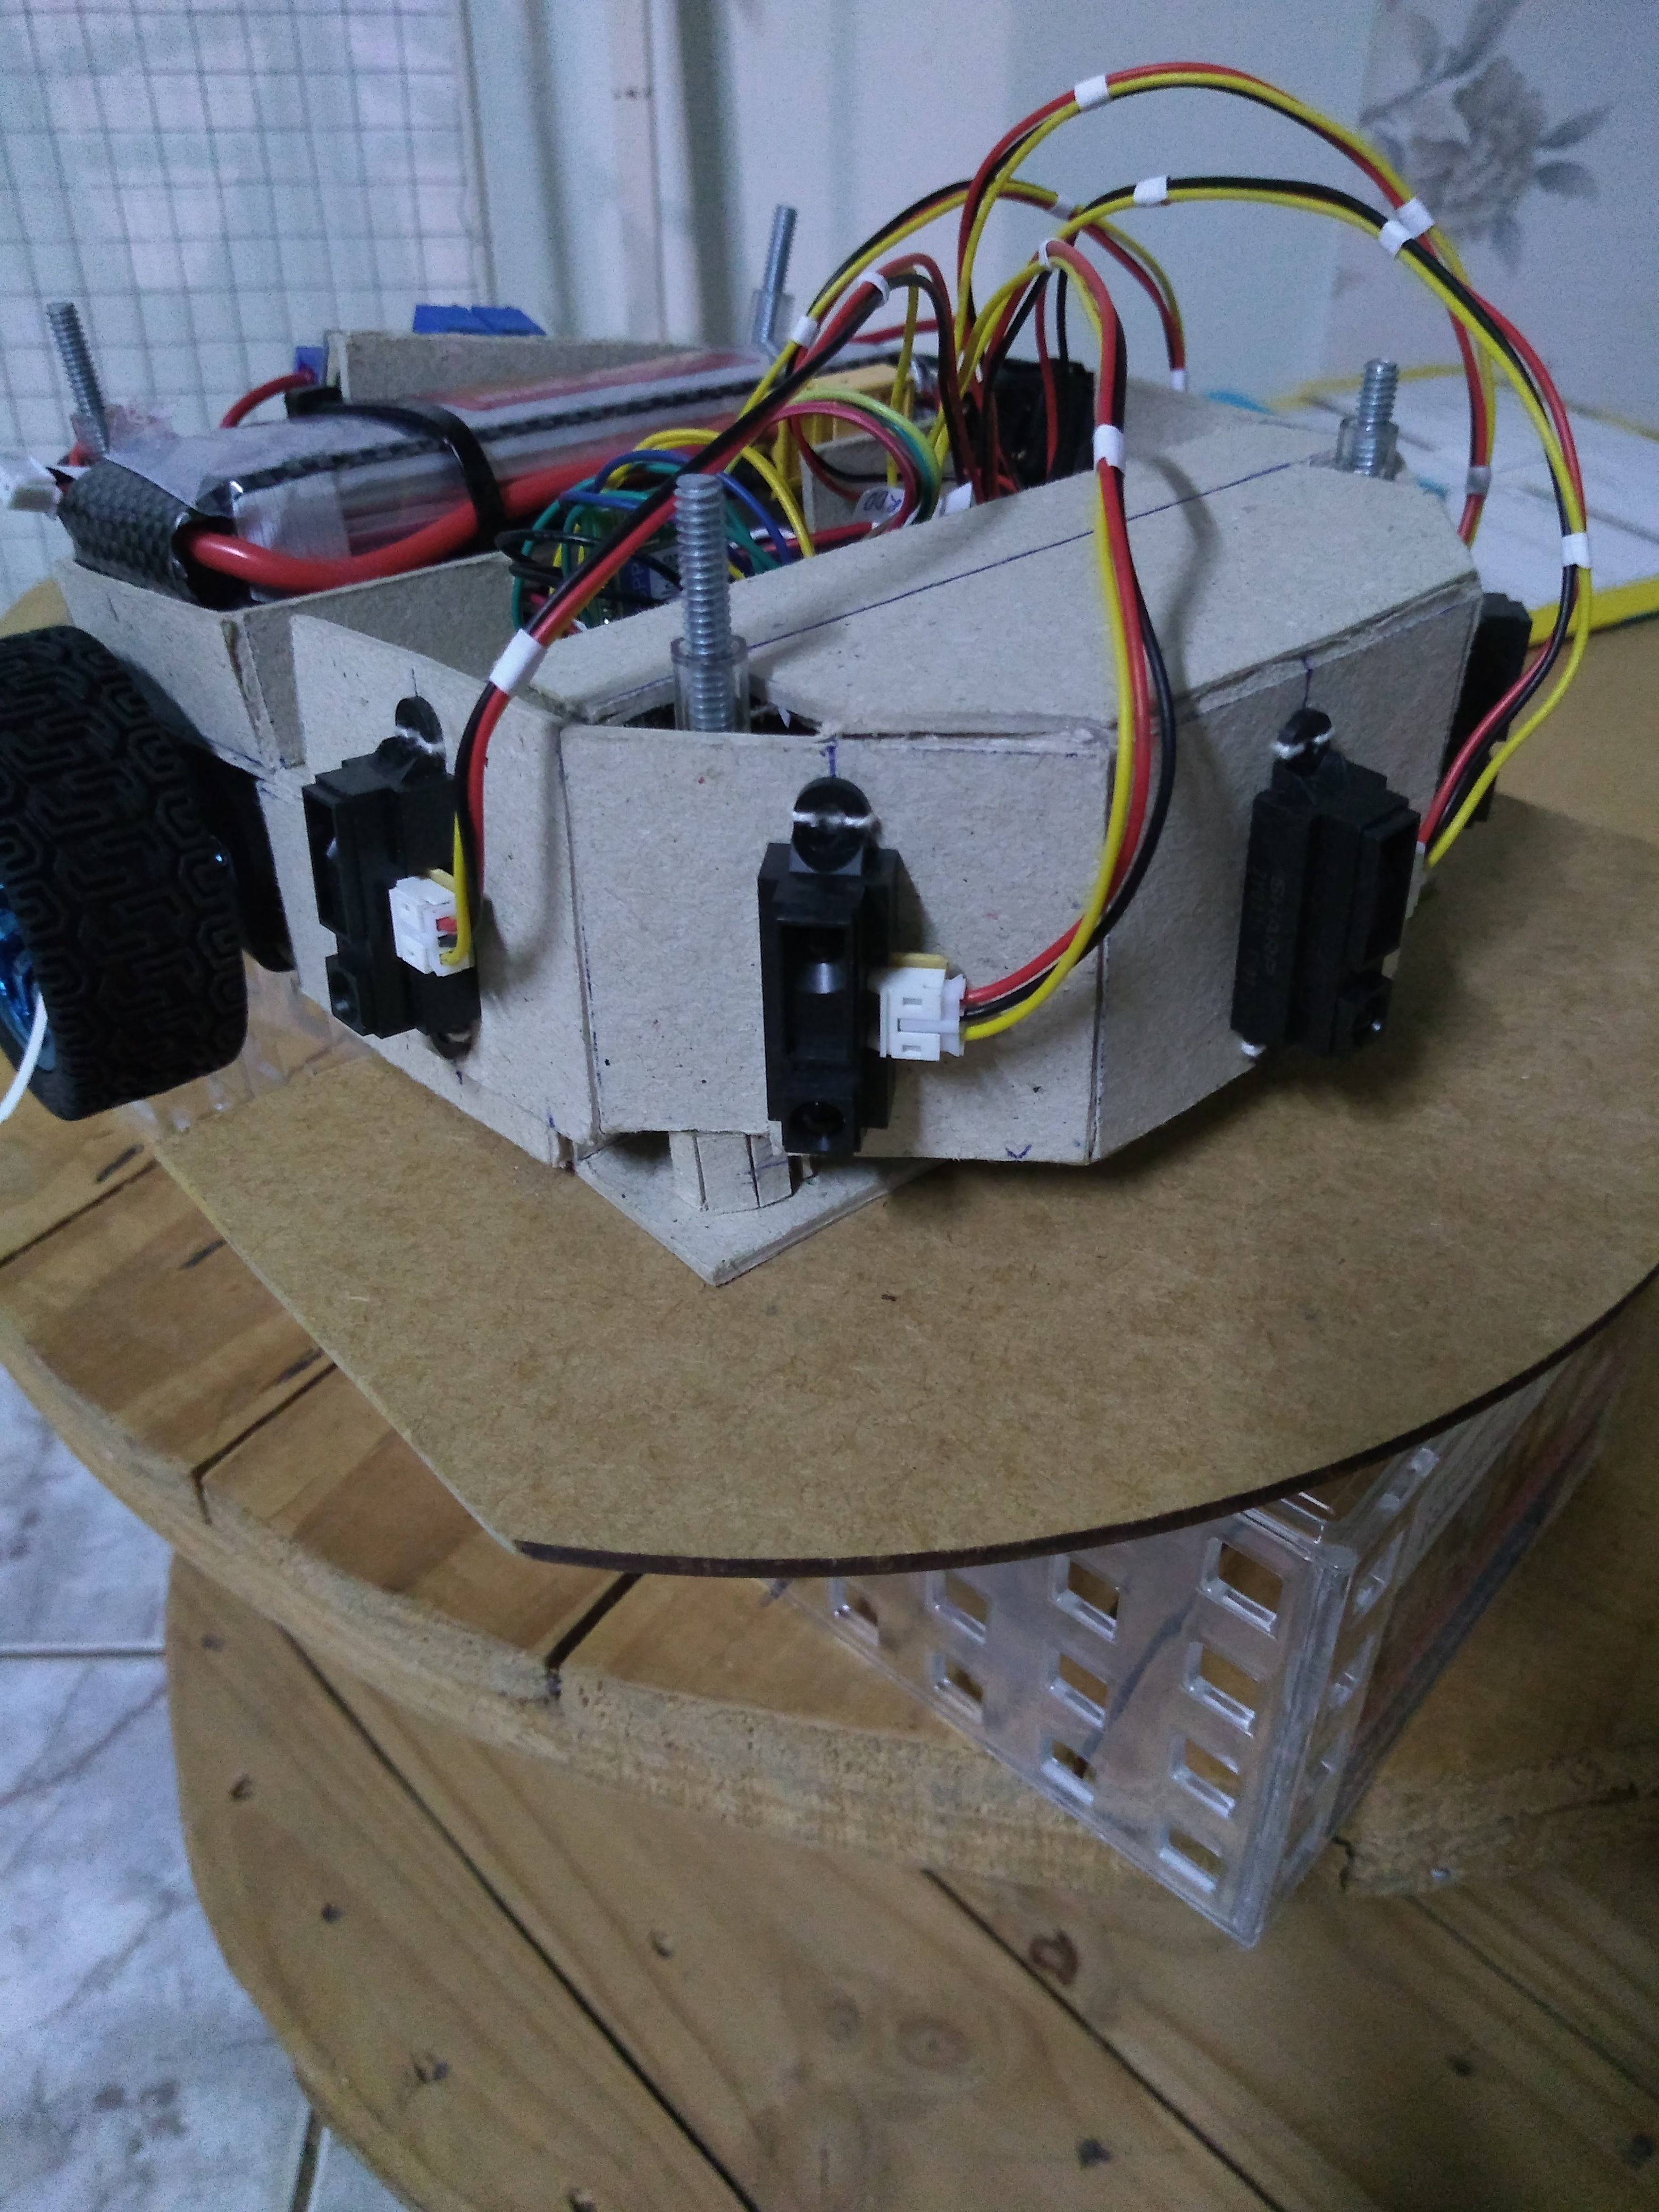
\includegraphics[trim={0cm 35cm 0cm 0cm}, clip, 
		scale=0.055]{Figuras/RoboMontagem5}%
		\subcaption{Posição dos parafusos de rosca}%
	\end{subfigure}%
	~
	\begin{subfigure}[b]{0.49\textwidth}%
		\centering
		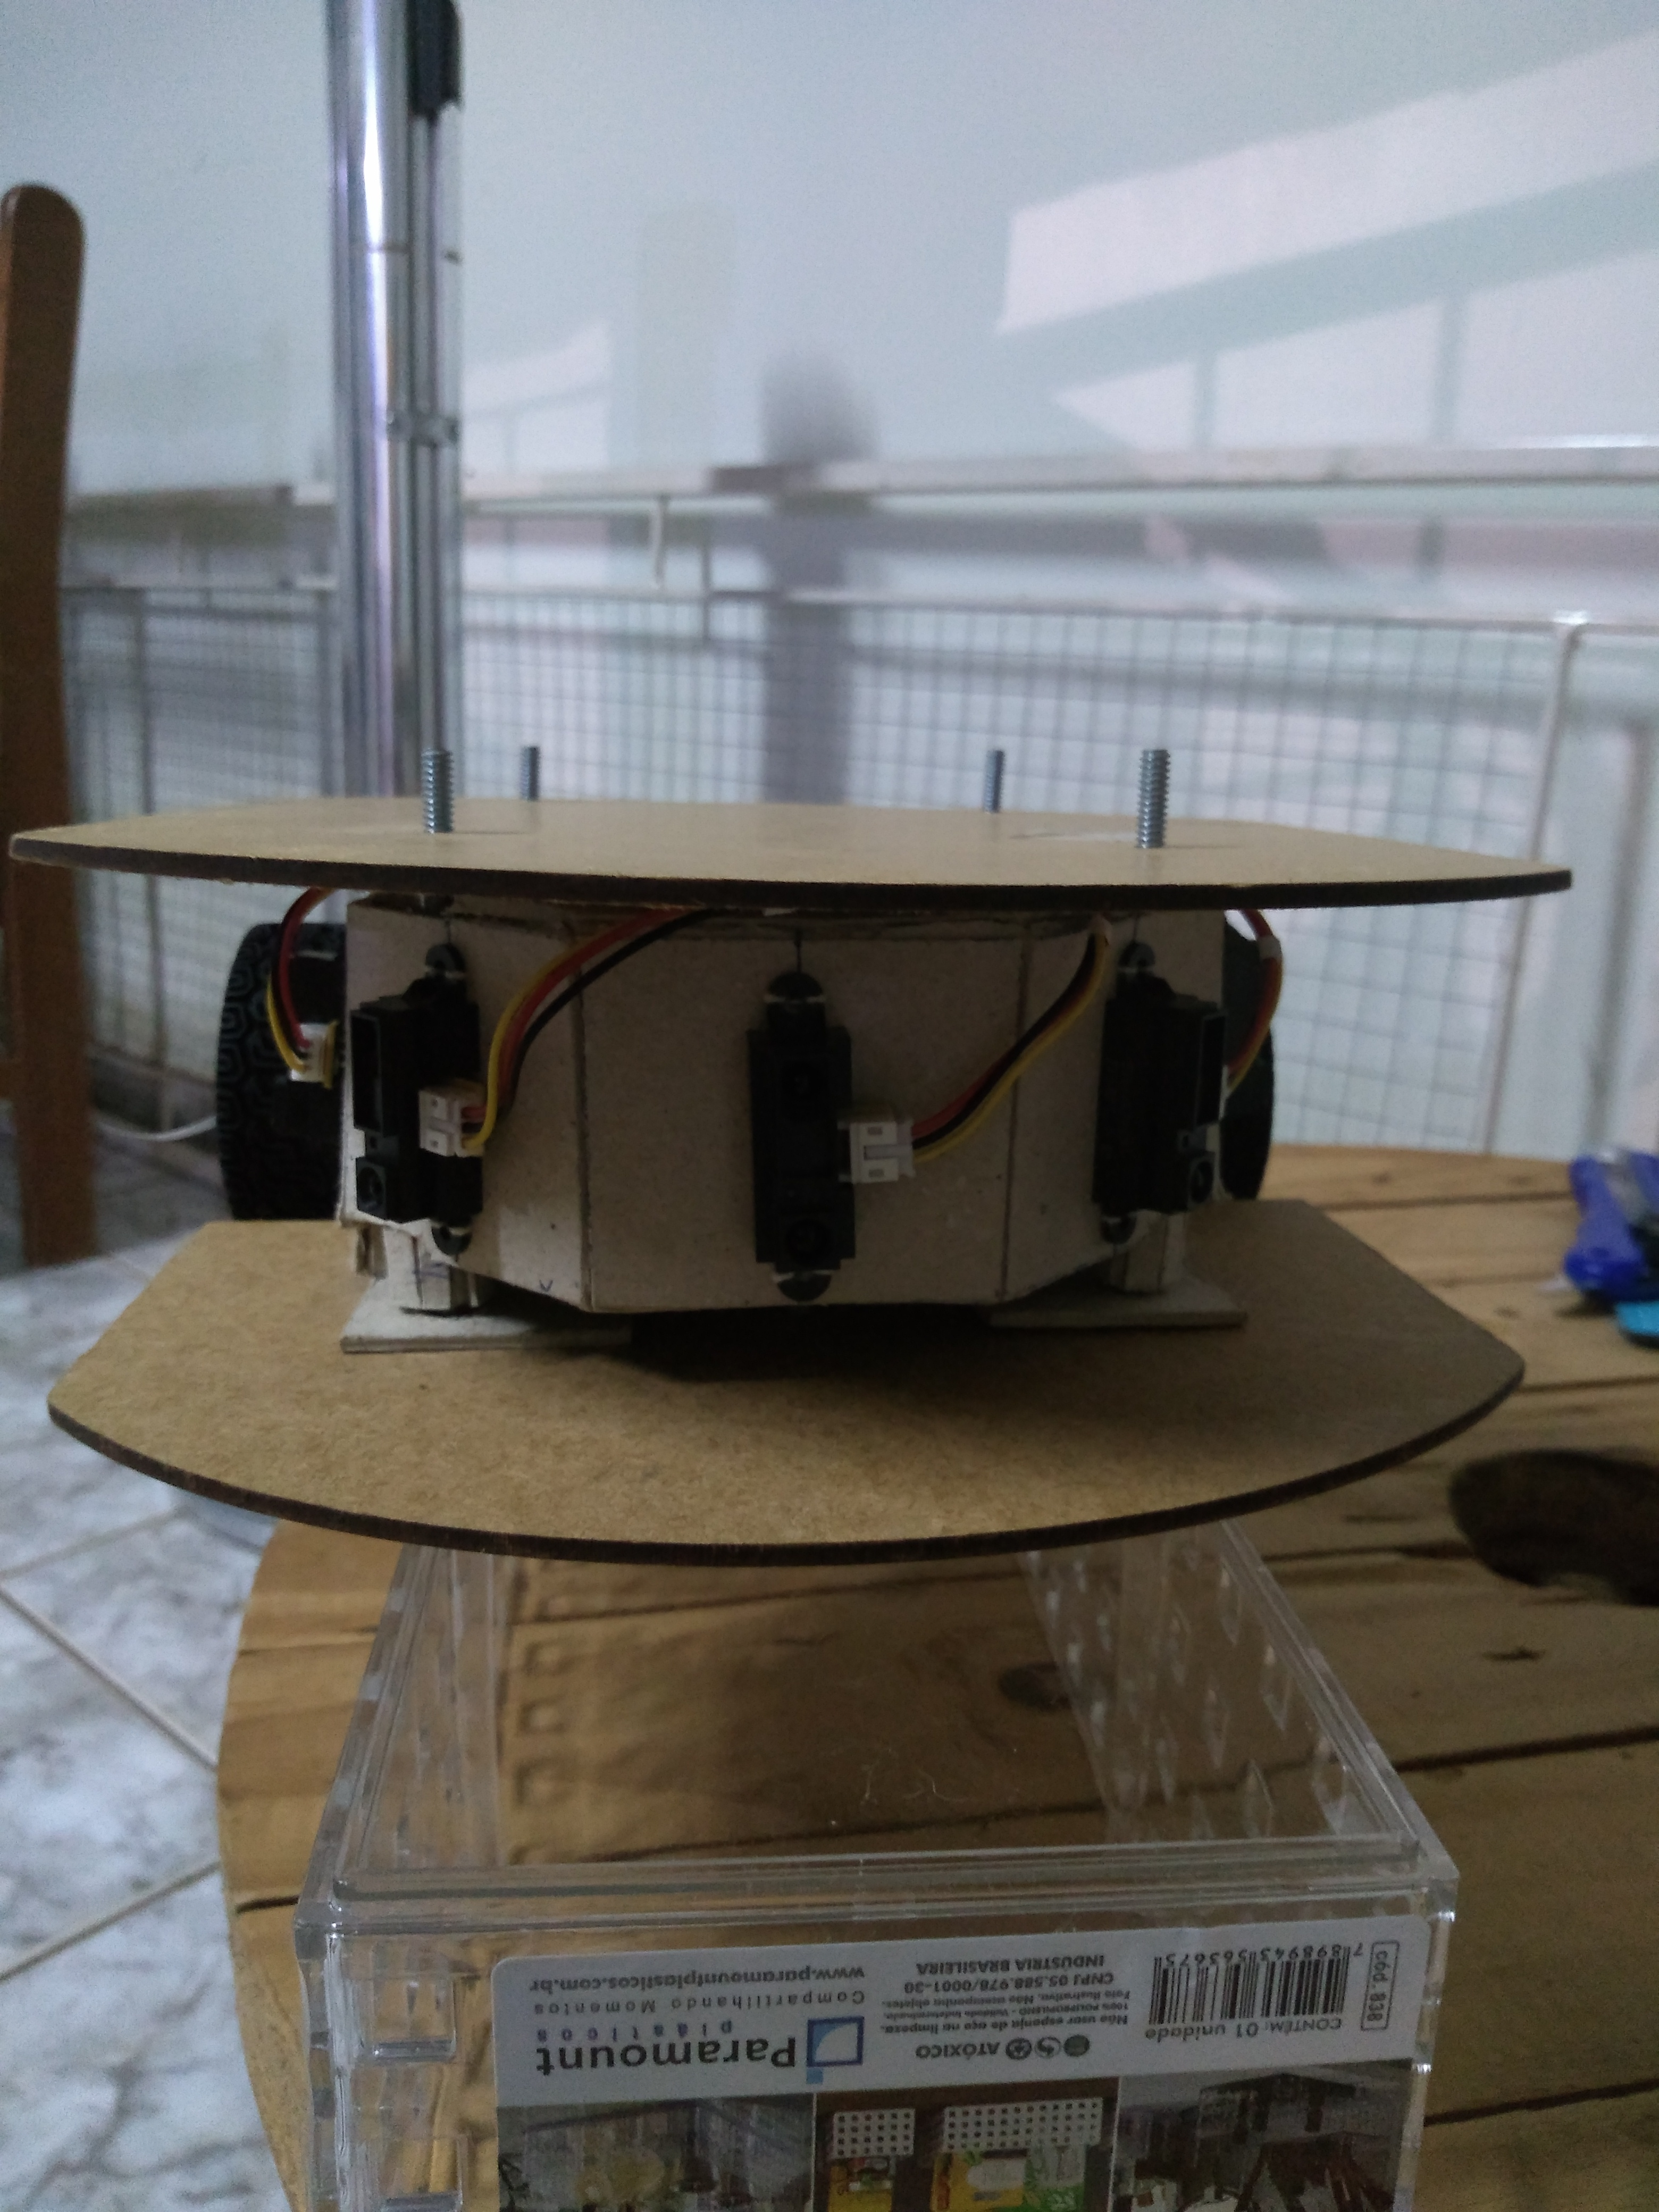
\includegraphics[trim={0cm 12.5cm 0cm 22.5cm}, clip, 
		scale=0.055]{Figuras/RoboMontagem6}%
		\subcaption{Robô montado}%
	\end{subfigure}%
\end{figure}